\documentclass[thesis]{deutez}
%%My_library 
\usepackage{placeins}%resim kaymaları için kullanıldı
\usepackage{amsmath,amsthm,mathtools}
\usepackage{listings}
\lstdefinestyle{customc}{
	belowcaptionskip=1\baselineskip,
	breaklines=true,
	frame=L,
	xleftmargin=\parindent,
	language=C,
	showstringspaces=false,
	basicstyle=\footnotesize\ttfamily,
	keywordstyle=\bfseries\color{green!40!black},
	commentstyle=\itshape\color{purple!40!black},
	identifierstyle=\color{black},
	stringstyle=\color{orange},
}

\lstdefinestyle{customasm}{
	belowcaptionskip=1\baselineskip,
	frame=L,
	xleftmargin=\parindent,
	language=Python,
	basicstyle=\footnotesize\ttfamily,
	commentstyle=\itshape\color{purple!40!black},
}

\lstset{escapechar=@,style=customc}
%%Images
\graphicspath{ {/home/rabikkk/Pictures/images/} }

%-------------------------------------%%

\watermarklogo{Deu.jpg}  % Dokuz Eylül Üniversitesi Logosu; Sayfaya arkasına varsayılan logo olarak basılır.
\projectname{Smart Mirror Controller}%
\ogrencininadi{Rabia DOĞAN}%
\advisor{Ph.D. Özgür TAMER}%
\jurya{Prof. Dr. Gülay TOHUMOĞLU}
\juryb{Ph.D. Abdül BALIKCI}
\chair{Prof. Dr. Mehmet KUNTALP}
\time{January,2021}%

\begin{document}

\begin{abstract}
		
\end{abstract}

\begin{ozet}
	
\end{ozet}
 
\tableofcontents
\listoftables
\listoffigures

\start

\chapter{INTRODUCTION}

\chapter{TECHNICAL BACKGROUND}

\section{Introduction to Artificial Neural Networks}

\section{Model Architecture for LE-NET5}
\begin{figure}[h!]
	\centering
	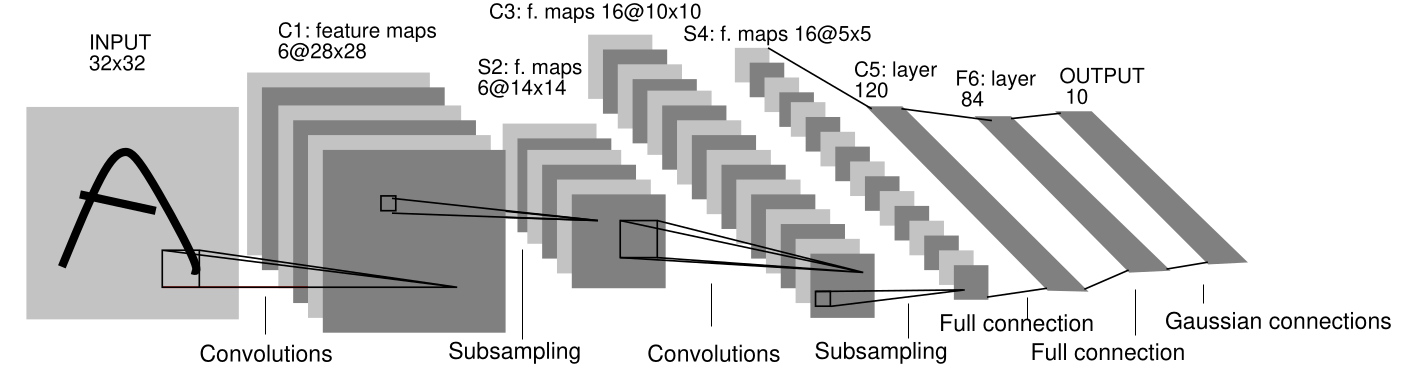
\includegraphics[width=1\textwidth]{lenet}
	\caption{Architecture of LeNet-5, a Convolutional Neural Network, here for digits recognition. Each plane is a feature map, i.e. a set of units
		whose weights are constrained to be identical.}
\end{figure}
\FloatBarrier
LeNet-5 A total of seven layers, each with no input with trainable parameters; each layer has multiple FeatureMap, which is a property of each of the FeatureMap inputs extracted via a convolution filter, and then each FeatureMap has multiple neurons.\\
\textbf{C1 layer-convolutional layer:}\\
The first convolution operation is performed on the input image (using 6 convolution kernels of size 5*5) to obtain 6 feature maps of C1 (6 feature maps of size 28 28, 32-5 + 1 = 28). The size of the convolution kernel is 5, and there are 6 (5 * 5 + 1) = 156 parameters in total, where +1 indicates that a kernel has a bias. For convolution layer C1, each pixel in C1 is dependent on 5 of 5 pixels and 1 aberration in the input image, so there are 156 28 * 28 = 122304 links in total.\cite{lenet}\\
\textbf{S2 layer-pooling layer (downsampling layer):}\\
The pooling is done immediately after the first convolution. Pooling is done using 2 cores and S2, 14x14 (28/2 = 14) 6 feature maps are obtained. S2's pooling layer is a weighting coefficient plus an offset multiplied by the sum of the pixels in the 2*2 area in C1, and then the result is remapped. So each pooling core has two training parameters i.e. 2x6 = 12 training parameters but there are 5x14x14x6 = 5880 connections.\cite{lenet}\\
\textbf{C3 layer-convolutional layer:}\\
After the first pooling, the second convolution, the output of the second convolution is C3, 16 pieces of 10x10 feature maps, and the size of the convolution kernel is 5. The first 6 feature maps of C3 (corresponding to column 6 of the first). red box) connects to 3 feature maps connected to S2 layer and next 6 feature maps are connected to S2 layer 4 feature maps are connected, next 3 feature maps are connected to 4 feature maps are unconnected in S2 layer and last one is linked to all feature maps in S2 layer. The convolution kernel size is still 5x5, so there are 6 (3*5*5 + 1) + 6 (4*5*5 + 1) + 3 (4*5*5 + 1) +1 (6*5*5 + 1) = 1516 parameters. The image size is 10 10 so there are 151600 connections.\cite{lenet}\\
\textbf{S4 layer-pooling layer (downsampling layer):}\\
S4 is the pooling layer, the window size is still 2*2, a total of 16 feature maps and 16 10x10 maps of the C3 layer are pooled in units of 2x2 to get 16 5x5 feature maps. This layer has a total of 32 training parameters, 2x16, 5x5x5x16 = 2000 connections.\cite{lenet}\\
\textbf{C5 layer-convolution layer:}\\
The C5 layer is a convolution layer. Since the size of the 16 images of the S4 layer is 5x5, the size of the image formed after convolution is 1x1, which is the same as the size of the convolution kernel. This results in 120 convolution results. Each is linked to 16 maps from the previous level. So there are (5x5x16 + 1) x120 = 48120 parameters and there are also 48120 connections.\cite{lenet}\\
\textbf{F6 layer-fully connected layer:}\\
Layer 6 is a fully connected layer. The F6 layer has 84 nodes corresponding to a 7x12 bitmap, -1 means white, 1 means black, so the black and white of each symbol's bitmap corresponds to a code. The training parameters and number of connections for this layer is (120 + 1) x84 = 10164.\cite{lenet}\\
\section{Python Libraries for Project}

\subsection{OpenCV}

\subsection{Python-Peripherial}

\subsection{Numpy}

\chapter{MATERIALS AND METHODS}
\section{Htpa32x32d Thermopile Infrared Array}
The sensor chosen to be used in the project is HTPA32x32d thermopile array sensor.
HTPA32x32d thermopile array sensor 32x32 pixel, operates between -10 and 70 degrees,
provides I2C communication, has an internal EEPROM and provides an 8-bit data set.
EEPROM data contains calibration data for each pixel of the sensor.\\

\begin{figure}[h!]
	\centering
	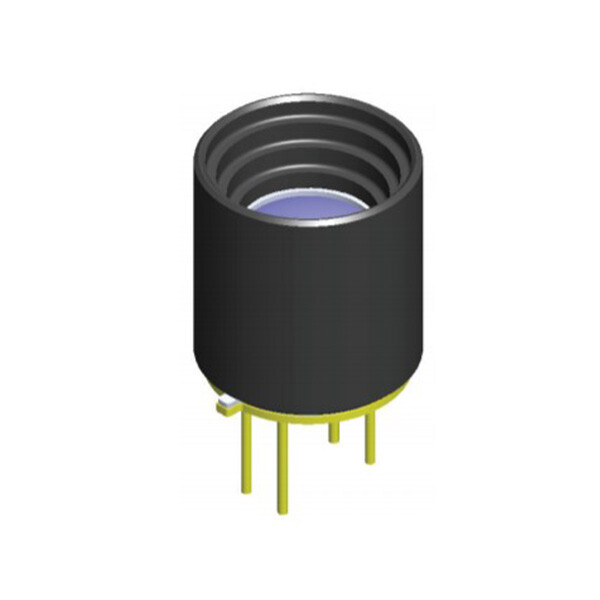
\includegraphics[width=0.35\textwidth]{htpa}
	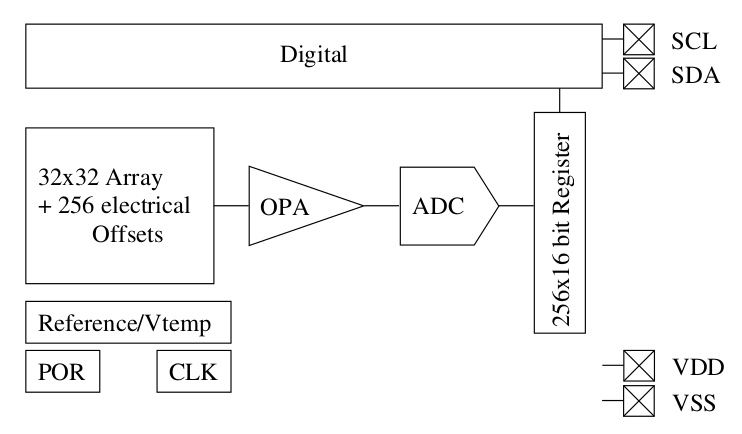
\includegraphics[width=0.5\textwidth]{htpasema}
	\caption{Schematic for HTPA32x32d}
\end{figure}
\FloatBarrier
	\begin{flushleft}
\begin{table}[h!]

	\caption{Genaral Features HTPA32x32d}
	\begin{tabular}{|l|l|l|l|l|}
		\hline
		Features\textbackslash\{\}& Sensitivity & Therm. Pix. Time Const. & Digital Interface & EEPROM Size\\\hline
		& 450V/W&$<4ms $& I2C & 64kBit  \\\hline
		Features\textbackslash\{\}& Max Frame&Field of View & Selectable Clock & Storage Temperature \\\hline
		&60 Hz& 33*33 deg & 1 to 13 Mhz & -40/85 Deg.C \\\hline
	\end{tabular}
\end{table}
\end{flushleft}
\FloatBarrier
\section{Sensor and MCU Communication PCB Design}
A mini card has been designed between the sensor and the Raspberry pi card to communicate. However, the card could not be printed. The card that will connect the sensor and the motherboard has been designed completely according to the standards recommended by Heimann company.\\
\begin{figure}[h!]
	\centering
	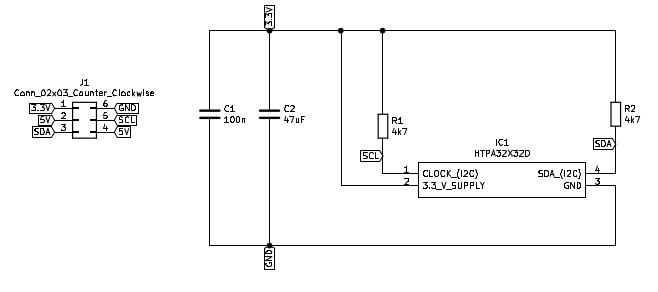
\includegraphics[width=0.6\textwidth]{schematic}
	\caption{Schematic Design of Communication PCB}
	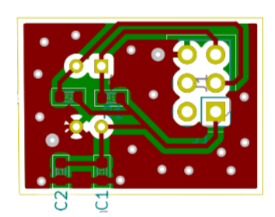
\includegraphics[width=0.4\textwidth]{pcb}
	\caption{PCB Design of Communication PCB}
\end{figure}
\FloatBarrier
In addition to this, we have produced a product suitable for a schematic on a mini perforated plate for use in communication with the card. In addition, we designed a protective cage from a 3d printer to protect the sensor.\\
\begin{figure}[h!]
	\centering
	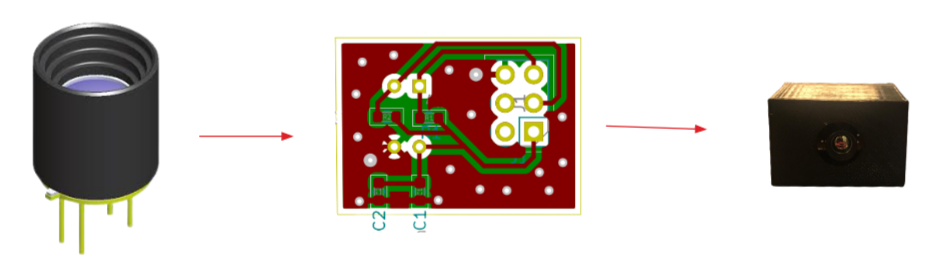
\includegraphics[width=1\textwidth]{mb}
	\caption{Mini Sensor Board}
\end{figure}

\section{Dataset}
\subsection{Multi-Modal Hand Gesture Dataset for Hand Gesture Recognition}
This dataset was created to validate a hand-gesture recognition system for Human-Machine Interaction (HMI). It is composed of 15 different hand-gestures (4 dynamic and 11 static) that are split into 16 different hand-poses, acquired by the Leap Motion device. Hand-gestures were performed by 25 different subjects (8 women and 17 men). Every gesture has 20 instances (repetitions) per subject, performed in different locations in the image.\cite{dataset}\\
for static and dynamic gestures:\\
This set contains 16 hand-poses, used for both static and dynamic hand-gestures:\\
A: L
B: fist moved
C: index
D: ok
E: C
F: heavy
G: hang
H: two
I: three
J: four
K: five
L: palm
M: down
N: palm moved
O: palm up
P: up
\begin{figure}[h!]
	\centering
	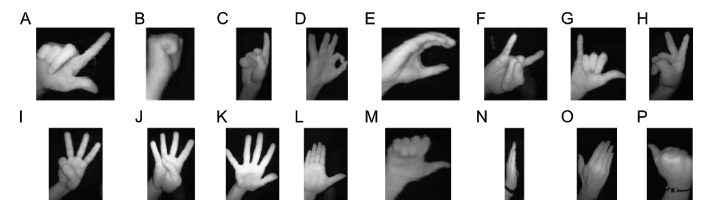
\includegraphics[width=0.8\textwidth]{data1.png}
	\caption{Hand Gesture Dataset}
\end{figure}
\FloatBarrier
\section{Data Augmentation}
Using this dataset, a new train and test set was created for the static gestures in the project. A total of 8000 and 2000 train and test sets were created with randomly selected images.However, both resizing and data augmentation were done in order to make the data set suitable for the project.\cite{aug}

\begin{figure}[h!]
	\centering
	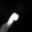
\includegraphics[width=0.2\textwidth]{close_test289}
	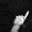
\includegraphics[width=0.2\textwidth]{index_test179}
	
\includegraphics[width=0.2\textwidth]{last_test71}
	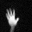
\includegraphics[width=0.2\textwidth]{open_test_0_9826}
	\caption{Close-Index-Last Page-Open Gestures}
\end{figure}
\FloatBarrier

\chapter{PROGRESS AND RESULT}
In this section, the methods to be applied in the project are included.

\begin{figure}[h!]
	\centering
	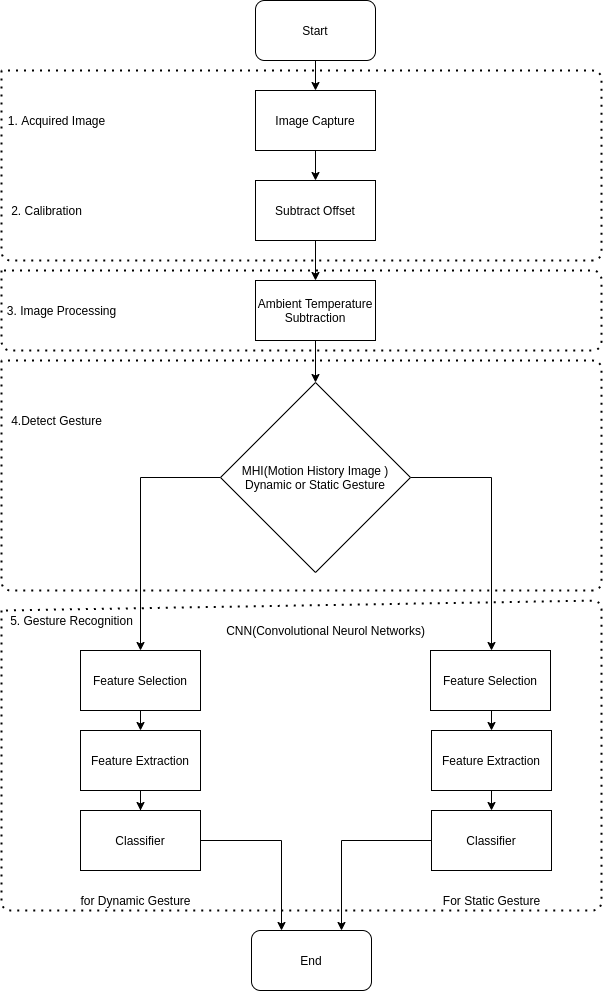
\includegraphics[width=0.75\textwidth]{sema}
	\caption{Software Flowchart}
\end{figure}
\FloatBarrier
\section{Capture Thermopiles Image}
\subsection{Heimann Thermopile Array Sensor communication}
First, I provided the connections between the sensor and the Raspberry Pi in order to receive the image. I provided the communication with the mini card I made in 4.2 using the I2C protocol.

With the device connected to a Raspberry Pi, and with the Pi configured.\cite{adaf} correctly for I2C, I was able to see the devices connected with the i2cdetect command.
\begin{figure}[h!]
	\centering
	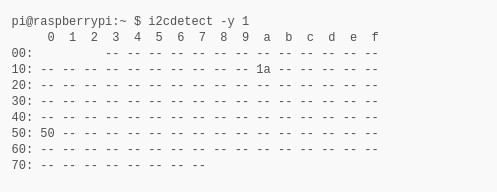
\includegraphics[width=0.8\textwidth]{raspi1.png}
	\caption{Thermopile Infrared Array Device and EEPROM Addresses}
\end{figure}
\FloatBarrier

In order to be able to read the data properly, the python-periphery\cite{perip} library was used. The sensor is divided into two parts (Top and Bottom Half), which are also divided into 4 blocks. The reading order is shown below for different blocks. When a conversion is initiated, the X Block of the upper and lower half are measured simultaneously. Each block consists of 128 Pixels sampled entirely in parallel. The reading order in the lower half is mirrored compared to the upper half so the center lines are always read last.

	\begin{table}[h!]
	\begin{center}
		\caption{Read Data 1 Command (Top Half of Array)}
		\begin{tabular}{|c|c|c|c|c|c|c|c|c|} 
			\hline
			Addr/CMD & \multicolumn{8}{c|}{0x1A (7 Bit!) / 0x0A}\\\cline{1-9}
			Read Data &7&6&5&4&3&2&1&0\\
			\cline{1-9}
			1. Byte / 2. Byte & \multicolumn{8}{c|}{PTAT 1 MSB / LSB or Vdd 1 MSB / LSB}\\\cline{1-9}
			3. Byte / 4. Byte & \multicolumn{8}{c|}{Pixel (0+BLOCK*128) MSB / LSB}\\\cline{1-9}
			5. Byte / 6. Byte & \multicolumn{8}{c|}{Pixel (1+BLOCK*128) MSB / LSB}\\\cline{1-9}
			... & \multicolumn{8}{c|}{}\\\cline{1-9}	
			257. Byte / 258. Byte & \multicolumn{8}{c|}{Pixel (127+BLOCK*128) MSB / LSB}\\\cline{1-9}
			
		\end{tabular}
	\end{center}
\end{table}
\FloatBarrier
\begin{table}[h!]
	\begin{center}
		\caption{Read Data 2 Command (Bottom Half of Array)}
		\begin{tabular}{|c|c|c|c|c|c|c|c|c|} 
			\hline
			Addr/CMD & \multicolumn{8}{c|}{0x1A (7 Bit!) / 0x0B}\\\cline{1-9}
			Read Data &7&6&5&4&3&2&1&0\\
			\cline{1-9}
			1. Byte / 2. Byte & \multicolumn{8}{c|}{PTAT 2 MSB / LSB or Vdd 2 MSB / LSB}\\\cline{1-9}
			3. Byte / 4. Byte & \multicolumn{8}{c|}{Pixel (992-BLOCK*128) MSB / LSB}\\\cline{1-9}
			5. Byte / 6. Byte & \multicolumn{8}{c|}{Pixel (993-BLOCK*128) MSB / LSB}\\\cline{1-9}
			... & \multicolumn{8}{c|}{}\\\cline{1-9}	
			65. Byte / 66. Byte & \multicolumn{8}{c|}{Pixel (1023-BLOCK*128) MSB / LSB}\\\cline{1-9}
			
			65. Byte / 66. Byte & \multicolumn{8}{c|}{Pixel (1023-BLOCK*128) MSB / LSB}\\\cline{1-9}
			
			67. Byte / 68. Byte & \multicolumn{8}{c|}{Pixel (960-BLOCK*128) MSB / LSB}\\\cline{1-9}
			
			69. Byte / 70. Byte & \multicolumn{8}{c|}{Pixel (961-BLOCK*128) MSB / LSB}\\\cline{1-9}
			
			... & \multicolumn{8}{c|}{}\\\cline{1-9}
			
			129. Byte / 130. Byte & \multicolumn{8}{c|}{Pixel (991-BLOCK*128) MSB / LSB}\\\cline{1-9}
			
			131. Byte / 132. Byte & \multicolumn{8}{c|}{Pixel (928-BLOCK*128) MSB / LSB}\\\cline{1-9}
			
			...& \multicolumn{8}{c|}{}\\\cline{1-9}
			
			257. Byte / 258. Bytes& \multicolumn{8}{c|}{Pixel (927-BLOCK*128) MSB / LSB}\\\cline{1-9}
			
		\end{tabular}
	\end{center}
\end{table}
\FloatBarrier
Each block is checked before it is read. The python-opencv\cite{cv2} library was used to visualize the obtained result.
\begin{figure}[h!]
	\centering
	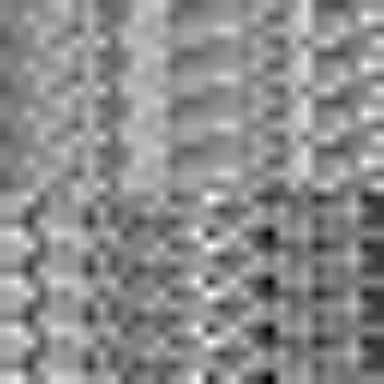
\includegraphics[width=0.23\textwidth]{4.img}
	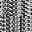
\includegraphics[width=0.23\textwidth]{3.img}
	\caption{Thermal Image}
\end{figure}
\FloatBarrier


Each pixel (or each analog-to-digital converter, given the repeating structure corresponding to each "block" of the sensor) has its own offset and sensitivity to incident light. Without calibrating it, this constant "noise" suppresses the signal from changing IR/temperature conditions. By subtracting the two frames in quick succession, this common noise signal is removed.

However, it is still quite noisy, as this frame subtraction increases random noise (since we now have contributions from two frames) and does not correct pixel-dependent sensitivity.
Only fabrication calibration will be done with EEPROM data in the next step.

\subsection{Calibrating images from Heimann Thermopile Array Sensor}

After reading an image off a Heimann thermopile array, the pixel values can be converted to temperature readings through the use of calibration parameters stored on the device. To extract the calibration parameters, it is easiest to first read off the entire EEPROM on the thermopile array.

\begin{figure}[h!]
	\centering
	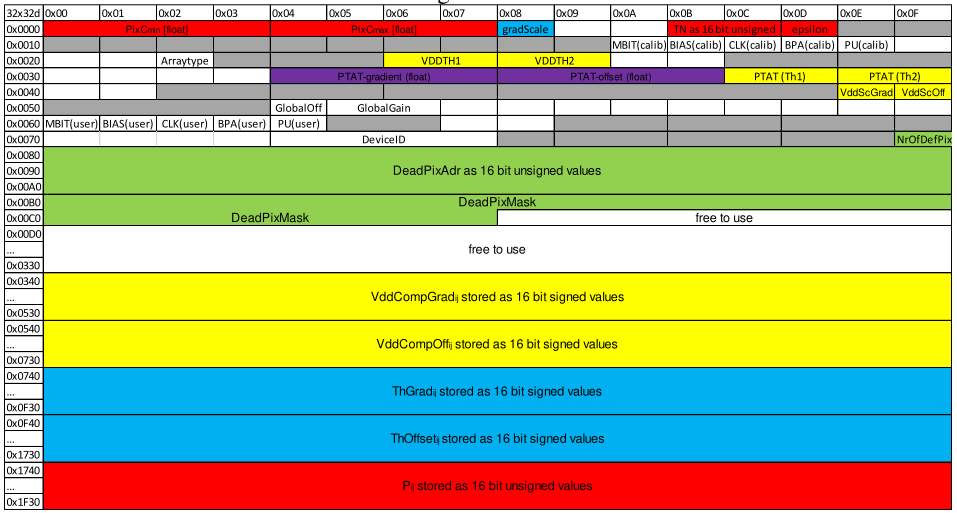
\includegraphics[width=1\textwidth]{eeprom}
	\caption{EEPROM overview 32x32d\cite{datasheet}}
\end{figure}
\FloatBarrier
Then, parameters and calibration values can be extracted from this array, as described in the Heimann datasheet.\cite{datasheet}\\
Calibration for only one pixel is done as follows.\\
$PTAT_{av} = \frac{\sum \limits _{i=0}^{7}{PTAT_i}}{8}=38152 Digits $ \\
$PTAT_{gradient}=0.0211 dK/Digit $ and $PTAT_{offset}=2195.0dK$ \\
$ V_{00}=34435 Digits $\\
$ elOffset[0]=34240 $\\
$gradScale=24  $\\
$ThGrad_{00}=11137$ \\
$ThOffset_{00}=65506 $\\
$VDD_{av}=35000 $\\
$ VDD_{TH1}= 33942 $\\
$ VDD_{TH2} = 36942 $\\
$ PTAT_{TH1} = 30000  $\\
$ PTAT_{TH_2} = 42000  $\\
$ VddCompGrad[ 0 ] = 10356 $\\
$ VddCompOff[ 0 ] =51390  $\\
$ VddScGrad = 16 $\\
$VddScOff = 23  $\\
$ PixC_{00}= 1\cdot087\cdot10^8 $\\
$ PCSCALEVAL = 1\cdot10^8 $\\
Calculation of ambient temperature:\\
$ 	T_a=PTAT_{av} \cdot PTAT_{gradient}+ PTAT_{offset}=38152 \cdot 0.0211 + 2195.0 dK =3000 dK $\\
Compensation of thermal offset:\\
$V_{00\_Comp}=V_{00}-\frac{Th_{Grad00} \cdot T_a}{2^{gradScale}}-Th_{Offset_{00}}=34439 $\\
Compensation of electrical offset:\\
$ 	V_{00\_Comp}^{\ast} =V_{00\_Comp}-elOffset[0]=199 $\\
Compensation of supply voltage:\\
$ V_{00-VDD_{Comp}}=V_{00\_Comp}^{\ast}-\frac{\frac{Vdd_{CompGrad}[0]\cdot PTAT_{av}}{2^{Vdd_{ScGrad}}}+V_{Vdd_{Compoff}}[0]}{2^{Vdd_{ScOff}}}\\
	\cdot(VDD_{av}-VDD_{TH1}-(\frac{VDD_{TH2}-VDD_{TH1}}{PTAT_{TH2}-PTAT_{TH1}})\cdot(PTAT_{av}-PTAT_{TH1}))=199-1=198 $
The sensitivity coefficients ( PixC ij ) are calculated:\\
$PixC_{00}=(\dfrac{P_{00} \cdot (PixC_{Max}-PixC_{Min})}{65535}+PixC_{Min}) \cdot \frac{epsilon}{100} \cdot \frac{GlobalGain}{100000}=1\cdot087\cdot10^8 $\\
Leading to a compensation of the pixel voltage:\\
$V_{00PixC}=\dfrac{	V_{00-VDD_{Comp}}\cdot PCSCALEVAL}{PixC_{0}}=182$\\ 

All operations are applied for 1024 pixels. Application result images are as in figure 4.4.

\begin{figure}[h!]
	\centering
	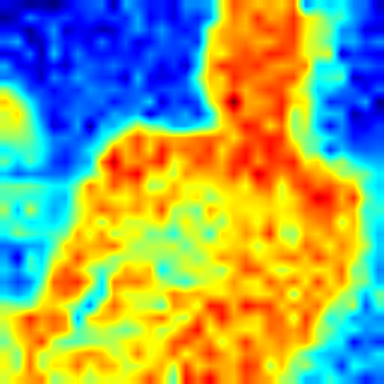
\includegraphics[width=0.23\textwidth]{last_test58}
	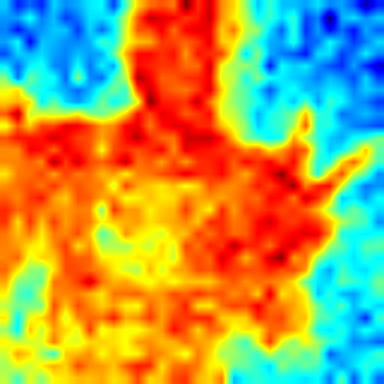
\includegraphics[width=0.23\textwidth]{last_test59}
	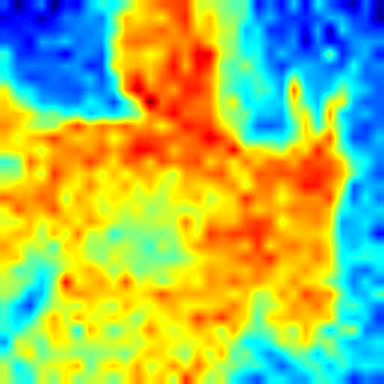
\includegraphics[width=0.23\textwidth]{last_test60}
	\caption{Thermal Images with EEPROM Calibration Data}
\end{figure}
\FloatBarrier
\paragraph~	\textbf{NOTE:All steps to acquired the image are made with reference to the datasheet\cite{datasheet}.}
\section{Hand Thermal Image Isolation}
The hand was isolated from the background without using any image processing method. For this, it has been arranged in a way that can remove the ambient temperature of the device from the image before giving a command. First, the average of 10 images was taken and given to all images. Thus, the background temperature was isolated.
\begin{figure}[h!]
	\centering
	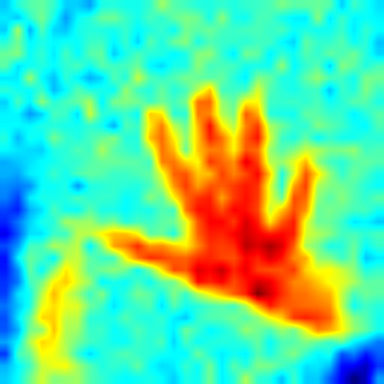
\includegraphics[width=0.23\textwidth]{rgb0}
	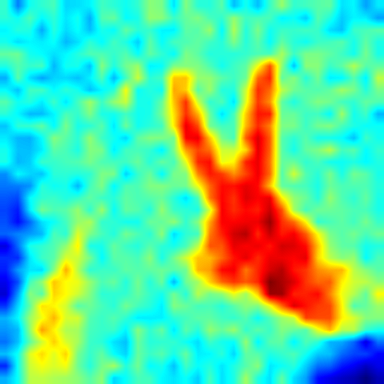
\includegraphics[width=0.23\textwidth]{rgb1}
	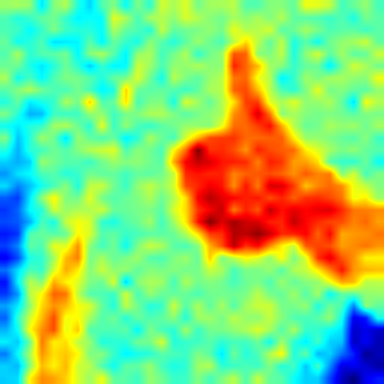
\includegraphics[width=0.23\textwidth]{rgb2}
	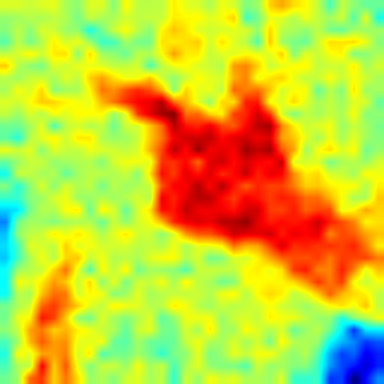
\includegraphics[width=0.23\textwidth]{rgb3}
	\caption{Thermal Images with Background}
\end{figure}

\section{Hand Gesture Recognition}
\subsection{Static Gesture Recognition}
\begin{figure}[h!]
	\centering
	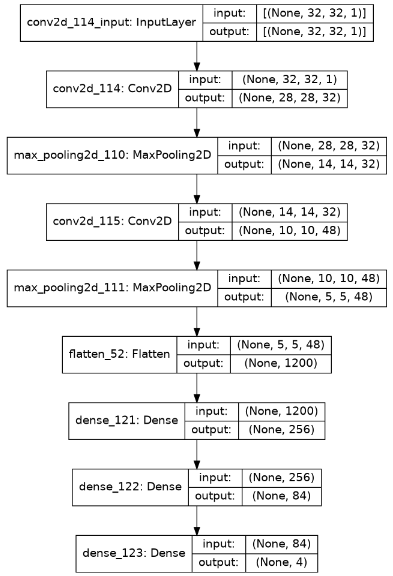
\includegraphics[width=0.5\textwidth]{model}
	\caption{Software Flowchart}
\end{figure}
\FloatBarrier
\subsubsection{Model Architecture for LE-NET5}
\subsubsection{Test Sets and Results}
\subsection{Dynamic Gesture Recognition}

\begin{table}[h!]
	\begin{center}
		\caption{Trim Register 1 (write only)\cite{datasheet}}
		\begin{tabular}{|c|c|c|c|c|c|c|c|c|}
			\hline
			Addr / CMD & \multicolumn{8}{c|}{0x1A (7 Bit!) / 0x03} \\
			\hline
			Trim Reg 1 & 7 & 6 &5  &4  &3  &2  &1&0  \\
			\hline
			Name & \multicolumn{2}{c|}{RFU} & \multicolumn{2}{c|}{REF\_CAL}& \multicolumn{4}{c|}{MBIT TRIM}\\
			\hline
		\end{tabular}
	\end{center}
\end{table}
\FloatBarrier

REF\_CAL: selectable amplification
\\

MBIT\_TRIM: m = 4 to 12 (m+4) bit as ADC resolution\\

In order to get the maximum efficiency from the sensor, to set the ADC Resolution to 16 bits, m of 12 was determined according to the data in the table. Since the framerate was too low, it was decided to speed up by sacrificing quality, but the quality was too low, revealing that ADC resolution should not be compromised. According to the resolutions, the images are as in figure 2.\\
\begin{figure}[h!]
	\centering
	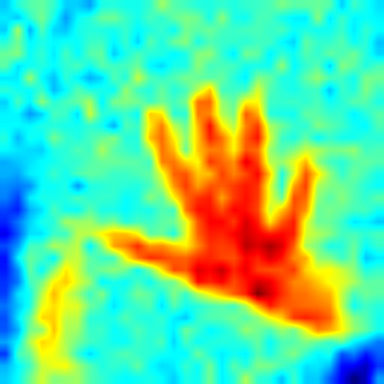
\includegraphics[width=0.23\textwidth]{rgb0}
	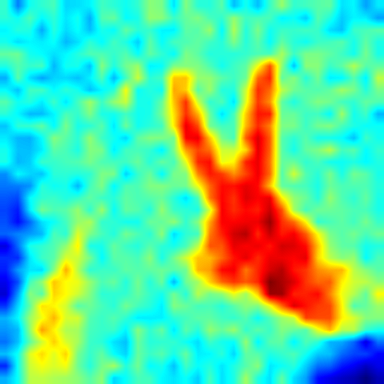
\includegraphics[width=0.23\textwidth]{rgb1}
	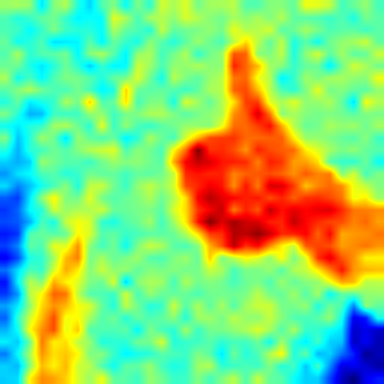
\includegraphics[width=0.23\textwidth]{rgb2}
	\caption{Thermal Images 8Bit-12Bit-16Bit ADC Resolution)}
\end{figure}
\begin{table}[h!]
	\begin{center}
		\caption{Trim Register 2 (write only)\cite{datasheet}}
\begin{tabular}{|c|c|c|c|c|c|c|c|c|}
	\hline
	Addr / CMD & \multicolumn{8}{c|}{0x1A (7 Bit!) / 0x04} \\
	\hline
	Trim Reg 1 & 7 & 6 &5  &4  &3  &2  &1&0  \\
	\hline
	Name & \multicolumn{3}{c|}{RFU} & \multicolumn{5}{c|}{BIAS TRIM TOP}\\
	\hline
\end{tabular}
	\end{center}
\end{table}
\FloatBarrier
BIAS\_TRIM\_TOP:0 to 31 $ \longrightarrow $ $ 1\mu A $ to $ 13 \mu A $\\

\begin{table}[h!]
	\begin{center}
		\caption{Trim Register 3 (write only)\cite{datasheet}}
		\begin{tabular}{|c|c|c|c|c|c|c|c|c|}
			\hline
			Addr / CMD & \multicolumn{8}{c|}{0x1A (7 Bit!) / 0x05} \\
			\hline
			Trim Reg 1 & 7 & 6 &5  &4  &3  &2  &1&0  \\
			\hline
	Name & \multicolumn{3}{c|}{RFU} & \multicolumn{5}{c|}{BIAS TRIM BOT}\\
			\hline
		\end{tabular}
	\end{center}
\end{table}
\FloatBarrier
BIAS\_TRIM\_BOT: 0 to 31 $ \longrightarrow $ $ 1\mu A $ to $ 13 \mu A $\\
This setting is used to adjust the bias current of the ADC. A faster clock frequency requires a
higher bias current setting.\cite{datasheet}\\

Having ADC resolution 16 made us think that it did not affect us much. Afterward, it was said that if the BIAS current value is set to the maximum, its speed may increase. However, as a result of this experiment, almost no change was observed in the framerate.\\

\begin{table}[h!]
	\begin{center}
		\caption{Trim Register 4 (write only)\cite{datasheet}}
		\begin{tabular}{|c|c|c|c|c|c|c|c|c|}
			\hline
			Addr / CMD & \multicolumn{8}{c|}{0x1A (7 Bit!) / 0x06} \\
			\hline
			Trim Reg 1 & 7 & 6 &5  &4  &3  &2  &1&0  \\
			\hline
			Name & \multicolumn{2}{c|}{RFU} & \multicolumn{6}{c|}{CLK TRIM}\\
			\hline
		\end{tabular}
	\end{center}
\end{table}
\FloatBarrier
CLK\_TRIM:0 to 63 $ \longrightarrow $ $ 1 MHz $ to $ 13 MHz $\\

The point where we could most easily observe the increase in Frame Rate was the Clock Trim set. Although I set the maximum value, I could not get the desired result here.\\
\section{Matching Gesture to Commands of Smart Mirror}

In the project carried out by Vestel, friends who are interested in the smart mirror part are expected to define the gestures for the android side of the smart mirror.

\chapter{COST ANALYSIS}
\chapter{CONCLUSION}
\chapter{APPENDIX}
\subsection{Capture Image from Htpa32x32d Thermopile Array Sensor}
\textbf{htpa32x32d Library}
\lstinputlisting[language=Python]{htpa_vsc.py}
\textbf{Capture Image}
\lstinputlisting[language=Python]{cap.py}
\subsection{Creating Dataset }
\textbf{Resize Dataset}\\
\lstinputlisting[language=Python]{resize.py}
\textbf{Dataset Augmentation}\\
\lstinputlisting[language=Python]{aug.py}
\subsection{Static Gesture Learning Algorithm}
\bibliographystyle{deueeebst2.bst}
\bibliography{fp_refs}

\end{document}